\chapter{GATE LEVEL SIMULATION}
\label{chap:gate_intro.tex}

In a typical VLSI design flow for verification, the first step after RTL level model of the design availabilty is writing behavioral test bench for functional verification. The functionally verified RTL goes through design synthesis during which it is mapped into low level design components in terms of primitives or logic gates. Synthesis is mostly an automated process using a ``{\it synthesizer}'' tool that converts RTL-level design source code into corresponding gate-level netlist mappings. This netlist is also called the pre-layout netlist.

The pre-layout netlist that was obtained from synthesis is then fed into a layout tool which maps the gate primities to silicon structures such as channels, gates, vias, etc. During this process certain modifications are done on netlist but it should not alter its functionality to its corresponding RTL. To validate this, another netlist called the post-layout netlist is generated back from the layed-out silicon structures by the layout tool itself. Validation is made by running LEC tool over both pre-layout and post-layout netlists or between post-layout netlist and RTL.

Though it would be ideal to use post-layout netlist for the purpose of gatesims, it would be too late in the design process. So work on gatesims starts with pre-layout netlist and progresses to pos-layout netlist as it becomes available. ~\figurename{~\ref{fig:gatesim.eps}} depicts progress of gatesim with respect to other design flows.
%% Meera : Need new flowchart. Use PPT, save as .tiff and convert to ps.

%\figurename{} 
\begin{figure}[H]
\centering
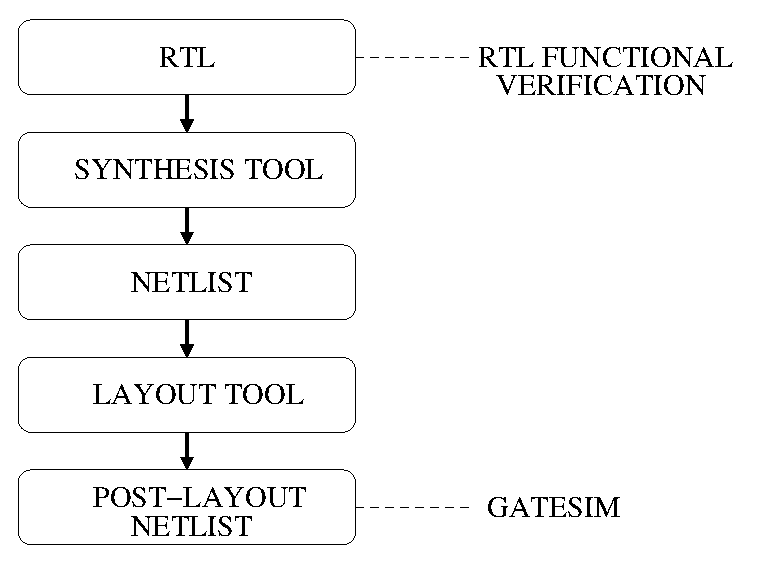
\includegraphics[width=3.5in]{./figures/gatesim.eps}
\caption{Design Flow}
\label{fig:gatesim.eps}
\end{figure}
Gate Level Simulation or Gatesim focuses on verifying the post layout netlist of the design. Gatesims are historically present from the days when designs were done with gates rather than at RTL abstraction. Verification with gates is a huge confidence booster before manufacturing of actual silicon as they are also thought to complement and cover gaps left by formal flow.


\section {NEED FOR GATESIM}
Gatesims are particularly effective for the following verification
\begin{itemize}
	\item[-]Power-up, reset propagation and initialization of the design
%% Naren:isitso?:	\item[-]The RTL written is synthesizable.
	\item[-]DFT structures those are absent in RTL and added during or after synthesis
	\item[-]non-resettable or un-initialized components such as memories
%% Naren:what?:	\item[-]The netlist passes all the critical test scenarios.
	\item[-]Power related circuits those are absent in RTL
	\item[-]Power switching verification
	\item[-]Dynamic power estimation
	\item[-]Validation of pessimistic behaviour of X-propagation in RTL simulation
	\item[-]Asynchronous interfaces those are false-paths in STA
	\item[-]Synchroniser logic and clock domain crossing verification
	\item[-]Analog-circuit and digital circuit co-verification
\end{itemize}

Finally, Gatesim is a great confidence-booster in ensuring the high quality of the netlist. It lowers the risk of finding late design, methodology or process issues.




\section{LIMITATIONS OF LEC AND STA}

Gatesims are targetted on post-layout netlist and that is almost clean of RTL bugs. The netlist also passes through couple of important verification steps such as Logic Equivalence Check (LEC) and Static Timing Analysis (STA), before it is targeted for Gatesims.

\emph {\bf LEC}: Logic Equivalence Checking (LEC) is a formal verification tool that compares a reference design against a derived design to prove equivalence or to report differences.  LEC does not require test patterns. Instead, LEC uses Boolean arithmetic techniques to prove equivalence between two design descriptions. Although LEC uses sophisticated formal algorithms to identify, map, and compare nodes in the netlists, the complexity is hidden from the user. %meera: what's this: [ieee].

\emph {\bf STA}: Static Timing Analysis does a input-independent timing analysis of the gate level netlist. It asserts if the circuit could operate flawless without timing issues. It computes the worst-case behaviour of the circuit, over all possible manufacturing variables. STA tools are at ease in handling a complex design with huge number of paths as they consider one path at a time (whether they are real or potential false paths). 



These formal static verification techniques are much faster and evolved than simulation based methods. However these verification methodologies, in spite of advancements in tools, cannot cover all aspects of required verification on netlist. Gatesim helps in filling up the gaps left by these methods. 

Limitations of LEC, which could be covered by Gatesims are:
\begin{itemize}
	\item Limitation of Static Equivalence Checking tools to catch all X-propagation or X-generation issues.
	\item Two-state methodologies can miss RTl-versus-netlist simulation and RTL-versus-RTL simulation differences.
	\item Incorrect mapping issues due to naming at sub-block level which can result in false pass. This will not be reported at the sub-block level LEC, but Gatesims can flag such incorrect connectivity.
\end{itemize}

Limitations of STA, which could be covered by Gatesims are:
\begin{itemize}
	\item \emph{\bf X-handling:} STA deals only with logic domain of logic-0 and logic-1. An X in the design cause undetermined values to propagate through the design. This cannot be checked with STA.
	\item \emph{\bf Interfaces between analog and digital blocks:} STA does not deal with analog blocks. And hence cannot verify connectivity between digital and analog blocks whereous Gatesims can.
	\item \emph{\bf Reset sequence:} Verifying that all flip-flops resets into their required logical value. STA cannot check this as certain declarations such as initial values on signal are not synthesizable and are verified only during simulation.
	\item \emph{\bf Asynchronous clock-domain crossings:} STA does not check if the correct clock synchronizers are being used.
\end{itemize}








%FIXME: Naren: Need to look at this section again
\section{ISSUES CAUGHT BY GATESIM}
%\section{DYNAMICALLY RECONFIGURABLE \\DATA-PATH}
The following are design issues missed initially but caught by gatesims:
\begin{enumerate}
		
	\item \emph{\bf X Squashing}

	X-Squashing is a term used when X-es get squashed in a simulation and don't propagate anymore through the logic. In one case there was an X-Squashing issue in behavioral RTL which led to a valid value being present in one of the RTL outputs during simulations, where as in gates X wasn't squashed and it propagated to the corresponding output resulting in a simulation mismatch between RTL and gates.

	\item \emph{\bf Reset X problem}

	Some of the un-initialized flops resulting in X issues were easily found during GLS.  After identifying such scenarios appropriate forces were added as part of Gate simulation flow.

	\item \emph{\bf Wrong connectivity during block level mapping}

	During integration, sub-blocks at top level may get connected incorrectly due to naming issues at the sub block level. Sub-block level LEC would not catch this issue, whereas gatesim flags the wrong connectivity.
\end{enumerate}







\section{ISSUES FACED BY GATESIM}
At system level, Gatesim is one of the most challenging verification task. This is because as design complexity increases, the limitations with gatesims become more prominent. Important difficulties associated with gate level simulation are:
\begin{itemize}


\item[-] Larger turn-around time (run, debug cycle).
\item[-] Limitation on size of netlist that can be verified through gatesim. This is an indirect cause due to larger build times and run times.
\item[-] Debugging the netlist simulation is challenging.
\item[-] Large compute and storage resource requirements. 

\end{itemize}

%FIXME: Naren: Need to solve issues faced is not well established
